\chapter{Neurônios, potenciais de ação e sinapses}\label{ch:b2:neurons-synapses}

Dê um toque no tendão abaixo da patela e a perna chuta, trinta
milissegundos depois. Nesse tempo, um estiramento foi percebido na
coxa, um sinal percorreu um metro até a medula espinal, atravessou uma
junção até uma segunda célula, percorreu um metro de volta e fez um
músculo se contrair --- a viagem de ida e volta inteira mais rápida que
um piscar de olhos. Nenhum \omterm{def:b2:cell-signalling:kinds}{hormônio} conseguiria fazer isso; isso é
feito por células construídas para conduzir, e por um sinal que não é
uma substância em movimento, mas uma onda de eletricidade regenerada ao
longo de uma membrana. Este capítulo trata dessa célula e desse sinal:
a tensão que um \omterm{def:b2:neurons-synapses:neuron}{neurônio} mantém através de sua membrana, o impulso que
ele dispara e como esse impulso se propaga, e a \omterm{def:b2:neurons-synapses:synapse}{sinapse}, onde o sinal
elétrico é transformado num sinal químico e de volta.

\section{O neurônio}

\begin{definition}[Neurônio, axônio, nervo]\label{def:b2:neurons-synapses:neuron}
\index{neurônio}\index{axônio}\index{dendrito}\index{mielina}\index{glia}
Um \emph{neurônio} é uma célula especializada na sinalização: um corpo
celular (o \emph{soma}), com o núcleo, \emph{dendritos} ramificados que
recebem sinais e um único \emph{axônio} --- um cabo de um a vinte
micrômetros de espessura e até um metro de comprimento --- que leva sua
saída a \emph{terminais} sobre outras células. O encéfalo humano tem
cerca de $10^{11}$ neurônios, e cada um faz cerca de mil \omterm{def:b2:neurons-synapses:synapse}{sinapses}. Os
neurônios são menos numerosos que a \emph{glia}: os astrócitos, que os
nutrem e tamponam seu meio, a micróglia, que os vigia, e as células que
envolvem os axônios em \emph{mielina} --- dezenas de voltas de sua
própria membrana, quase sem citoplasma, formando uma bainha isolante
interrompida mais ou menos a cada milímetro nos \emph{\omterm{prop:b2:neurons-synapses:myelin}{nós de Ranvier}}.
Um \emph{nervo} é um feixe de milhares de axônios, sensitivos e motores,
que correm juntos num tecido conjuntivo. Os neurônios não se dividem no
adulto (com poucas exceções), e um axônio separado de seu corpo celular
morre; um neurônio é uma célula que precisa durar a vida inteira.
\end{definition}

\begin{omfigure}
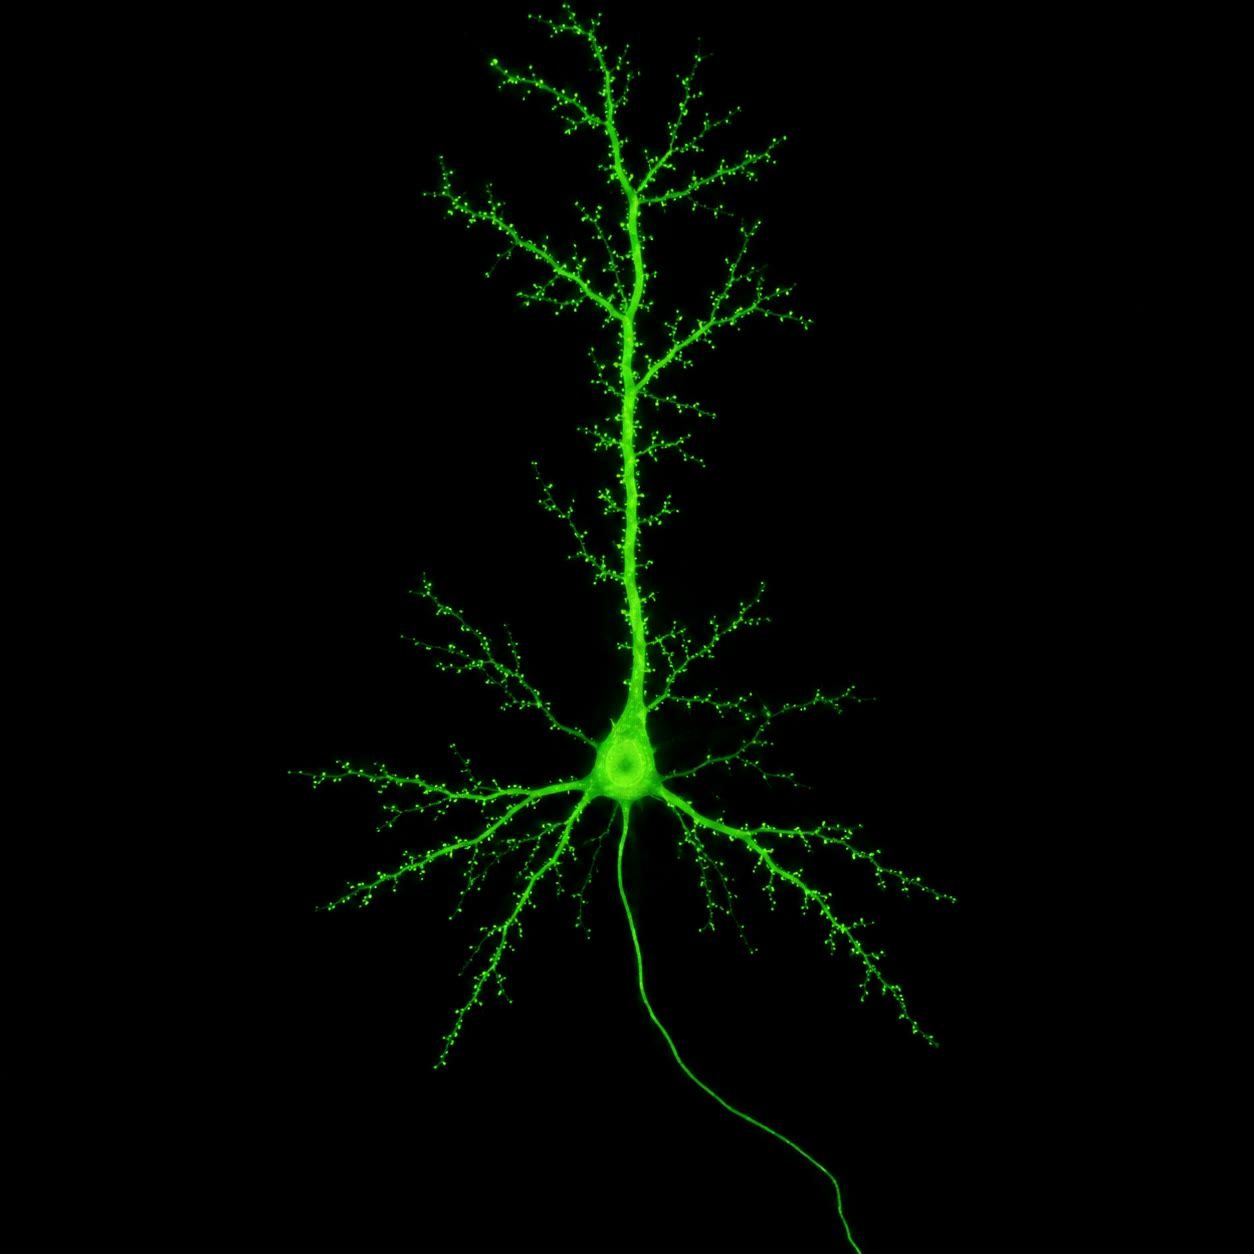
\includegraphics[width=0.4\linewidth]{images/book4/ai/b4-20-neuron-fluorescence.jpg}\hspace{0.05\linewidth}
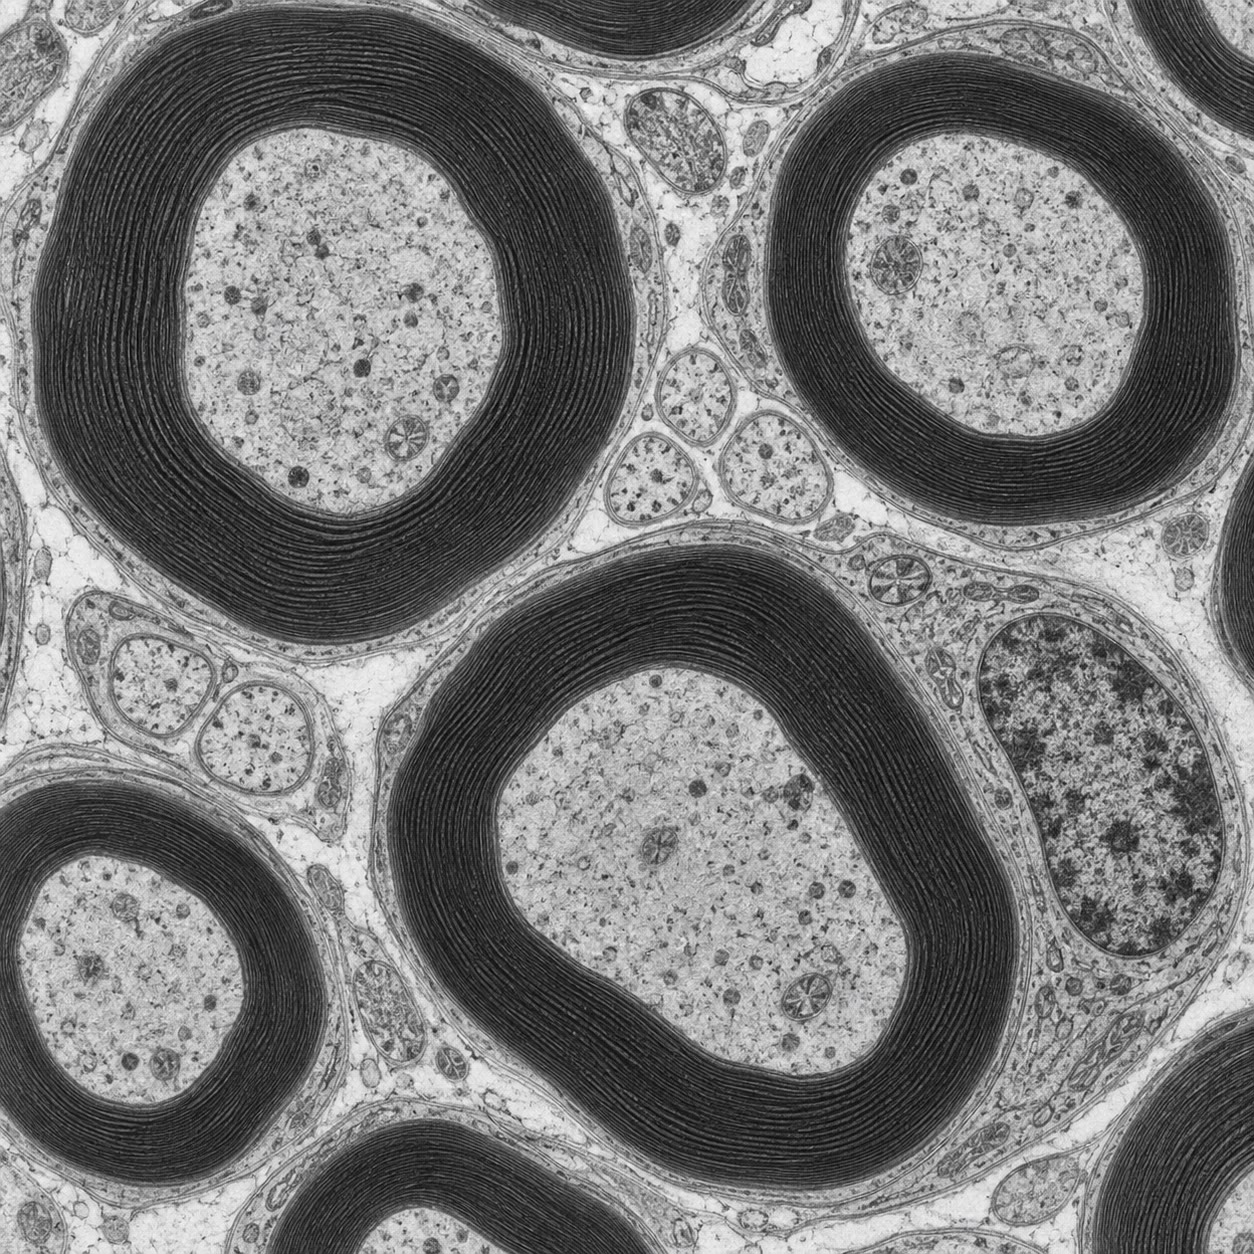
\includegraphics[width=0.4\linewidth]{images/book4/ai/b4-20-myelinated-axons-tem.jpg}

{\small À esquerda: um \omterm{def:b2:neurons-synapses:neuron}{neurônio} piramidal preenchido com corante --- o
corpo celular, os \omterm{def:b2:neurons-synapses:neuron}{dendritos} espinhosos que recebem e o \omterm{def:b2:neurons-synapses:neuron}{axônio} fino que
sai da base. À direita: \omterm{def:b2:neurons-synapses:neuron}{axônios} em corte transversal ao microscópio
eletrônico, cada um envolto na espiral escura de sua bainha de \omterm{def:b2:neurons-synapses:neuron}{mielina}.}
\end{omfigure}

\section{O potencial de repouso}

\begin{theorem}[O potencial de Nernst]\label{thm:b2:neurons-synapses:nernst}
\index{potencial de Nernst}\index{potencial de equilíbrio}
Uma membrana permeável a um único íon de carga $z$, que separa as
concentrações $c_{\text{ext}}$ e $c_{\text{int}}$, se estabiliza no
\emph{\omterm{thm:b2:neurons-synapses:nernst}{potencial de equilíbrio}} em que a força elétrica sobre o íon
equilibra sua difusão:
\[
E = \frac{RT}{zF}\ln\frac{c_{\text{ext}}}{c_{\text{int}}} \approx \frac{\qty{61.5}{mV}}{z}\log_{10}\frac{c_{\text{ext}}}{c_{\text{int}}} \quad (\qty{37}{\celsius}).
\]
Um \omterm{def:b2:neurons-synapses:neuron}{neurônio} mantém \qty{140}{mmol/L} de potássio dentro contra
\qty{5}{mmol/L} fora, e \qty{15}{mmol/L} de sódio dentro contra
\qty{145}{mmol/L} fora, gradientes construídos pela bomba de sódio e
potássio ao custo de um terço do ATP da célula. Daí
$E_{\mathrm K} = 61.5\log_{10}(5/140) = \qty{-89}{mV}$ e
$E_{\mathrm{Na}} = 61.5\log_{10}(145/15) = \qty{+61}{mV}$: se a
membrana deixasse passar apenas o potássio, ela ficaria a
\qty{-89}{mV}; se apenas o sódio, a \qty{+61}{mV}.
\end{theorem}
\begin{proof}
No equilíbrio, o potencial eletroquímico do íon é o mesmo dos dois
lados: $RT\ln c_{\text{int}} + zFV_{\text{int}} = RT\ln
c_{\text{ext}} + zFV_{\text{ext}}$, de modo que $V_{\text{int}} -
V_{\text{ext}} = (RT/zF)\ln(c_{\text{ext}}/c_{\text{int}})$. A
\qty{310}{K}, $RT/F = \qty{26.7}{mV}$ e $\ln 10 \times 26.7 =
\qty{61.5}{mV}$. (Deduzido no volume do Ano 1 a partir da distribuição
de Boltzmann; aqui apenas relembrado.)
\end{proof}

\begin{theorem}[O potencial de repouso como média ponderada]\label{thm:b2:neurons-synapses:chord}
\index{potencial de repouso}\index{condutância (membrana)}
Se a membrana conduz vários íons, cada um com uma condutância $g_i$ (a
facilidade com que ele passa, fixada pelo número de canais abertos), o
potencial estacionário em que as correntes se anulam é
\[
V = \frac{\sum_i g_i E_i}{\sum_i g_i},
\]
uma média dos \omterm{thm:b2:neurons-synapses:nernst}{potenciais de equilíbrio} ponderada pelas condutâncias. Em
repouso, a membrana de um \omterm{def:b2:neurons-synapses:neuron}{neurônio} é cerca de vinte vezes mais
permeável ao potássio que ao sódio, de modo que
$V \approx (20\times(-89) +
61)/21 = \qty{-82}{mV}$; contando o cloreto e os pequenos vazamentos, o
\omterm{thm:b2:neurons-synapses:chord}{potencial de repouso} é de \qty{-70}{mV}. A membrana repousa perto de
$E_{\mathrm K}$ porque os canais de potássio estão abertos; tudo o que
abre canais de sódio a arrasta em direção a $E_{\mathrm{Na}}$ --- e esse
é todo o princípio da sinalização nervosa.
\end{theorem}
\begin{proof}
Cada íon leva uma corrente $I_i = g_i(V - E_i)$ (lei de Ohm, com a força
motriz medida a partir do \omterm{thm:b2:neurons-synapses:nernst}{potencial de equilíbrio} do próprio íon). Num
potencial estacionário, a corrente total é nula: $\sum_i g_i(V - E_i) =
0$, donde $V\sum g_i = \sum g_iE_i$. (O tratamento completo, em que as
permeabilidades entram pela equação de Goldman--Hodgkin--Katz, dá a
mesma ponderação em primeira ordem.)
\end{proof}

\section{O potencial de ação}

\begin{proposition}[O impulso]\label{prop:b2:neurons-synapses:ap}
\index{potencial de ação}\index{canal dependente de voltagem}\index{limiar}\index{período refratário}
A membrana do \omterm{def:b2:neurons-synapses:neuron}{axônio} contém \emph{canais de sódio dependentes de
voltagem}, fechados em repouso e abertos pela despolarização. Se um
estímulo eleva o potencial de \qty{-70}{mV} além de um \emph{limiar}
perto de \qty{-55}{mV}, abrem-se canais suficientes para deixar entrar
mais sódio do que o vazamento de potássio consegue compensar; o
potencial sobe, mais canais se abrem e, em uma fração de milissegundo,
a membrana é levada em direção a $E_{\mathrm{Na}}$ --- uma
\emph{retroalimentação positiva} explosiva e de tudo ou nada. O pico
fica perto de \qty{+40}{mV} porque os canais de sódio se
\emph{inativam} até um milissegundo depois de se abrirem e porque
\emph{canais de potássio dependentes de voltagem}, mais lentos, se abrem
e levam o potencial de volta em direção a $E_{\mathrm K}$,
ultrapassando-o numa \emph{hiperpolarização} antes que os canais de
potássio se fechem. O \emph{\omterm{prop:b2:neurons-synapses:ap}{potencial de ação}} dura cerca de um
milissegundo; durante mais um ou dois milissegundos, os canais de sódio
inativados não conseguem se reabrir (o \emph{\omterm{prop:b2:neurons-synapses:ap}{período refratário}}), o que
limita a frequência de disparo a algumas centenas por segundo e obriga o
impulso a se propagar num único sentido. Por ser de tudo ou nada, o
impulso não leva nenhuma informação em sua amplitude: o \omterm{def:b2:neurons-synapses:neuron}{neurônio}
codifica a intensidade em sua \emph{frequência}. Cerca de $10^{4}$ íons
de sódio entram e o mesmo número de íons de potássio sai a cada impulso
--- uma mudança de concentração desprezível, restaurada pela bomba sem
pressa.
\end{proposition}
\begin{proof}[Evidências]
Hodgkin e Huxley (1952), usando o \omterm{def:b2:neurons-synapses:neuron}{axônio} gigante da lula (meio
milímetro de espessura, de modo que se podia introduzir um fio dentro
dele) e um amplificador com retroalimentação que mantinha o potencial
de membrana em qualquer valor escolhido (a \emph{fixação de voltagem})
enquanto registrava a corrente necessária para mantê-lo, separaram a
corrente num componente precoce de entrada, que desaparecia quando se
retirava o sódio do banho, e num componente tardio de saída, levado
pelo potássio; mediram como cada condutância subia e caía com o tempo
em cada voltagem; e, ajustando cada uma com algumas equações,
calcularam a forma, o limiar, a velocidade e o \omterm{prop:b2:neurons-synapses:ap}{período refratário} do
\omterm{prop:b2:neurons-synapses:ap}{potencial de ação} apenas a partir das duas condutâncias. Todas as
previsões se confirmaram. Os próprios canais foram vistos vinte e cinco
anos depois, um de cada vez, com o \textit{patch clamp}; a tetrodotoxina
(o veneno do baiacu) bloqueia o canal de sódio e abole o impulso, e o
tetraetilamônio bloqueia o canal de potássio e o prolonga.
\end{proof}

\begin{omfigure}
\begin{tikzpicture}
\begin{axis}[
  width=0.9\linewidth, height=6.4cm,
  axis x line=bottom, axis y line=left,
  xmin=0, xmax=4, ymin=-100, ymax=60,
  xlabel={tempo (ms)}, ylabel={potencial de membrana (mV)},
  xlabel style={font=\small, at={(axis description cs:0.5,-0.1)}, anchor=north},
  ylabel style={font=\small},
  tick label style={font=\small}, xtick={0,1,2,3,4}, ytick={-90,-70,-55,0,40},
  legend style={font=\scriptsize, at={(0.97,0.95)}, anchor=north east, draw=none},
  clip=false,
]
\addplot[very thick, omDef] coordinates {(0,-70) (0.4,-70) (0.5,-64) (0.6,-55) (0.7,-30) (0.8,10) (0.9,35) (1.0,40) (1.1,30) (1.2,10) (1.35,-20) (1.5,-50) (1.7,-75) (1.9,-85) (2.2,-82) (2.6,-76) (3.2,-71) (4,-70)};
\addlegendentry{potencial de membrana}
\addplot[thick, omThm, dashed] coordinates {(0,0) (0.5,0) (0.6,5) (0.7,20) (0.8,35) (0.9,30) (1.0,20) (1.1,8) (1.2,3) (1.4,0) (4,0)};
\addlegendentry{$g_{\mathrm{Na}}$ (relativa)}
\addplot[thick, omProp, dashed] coordinates {(0,0) (0.6,0) (0.8,2) (1.0,8) (1.2,16) (1.4,20) (1.7,17) (2.0,10) (2.4,4) (3.0,1) (4,0)};
\addlegendentry{$g_{\mathrm K}$ (relativa)}
\draw[dashed, gray] (axis cs:0,-55) -- (axis cs:4,-55); \node[font=\scriptsize, anchor=south east] at (axis cs:4,-55) {limiar};
\draw[dashed, gray] (axis cs:0,-89) -- (axis cs:4,-89); \node[font=\scriptsize, anchor=south east] at (axis cs:3.7,-89) {$E_{\mathrm K}$};
\draw[<->, gray] (axis cs:1.0,50) -- (axis cs:2.5,50); \node[font=\scriptsize, anchor=south, gray] at (axis cs:1.75,50) {refratário};
\end{axis}
\end{tikzpicture}

{\small Um \omterm{prop:b2:neurons-synapses:ap}{potencial de ação}. Além do limiar, a condutância ao sódio
(vermelho) sobe de modo explosivo e leva o potencial em direção a
$E_{\mathrm{Na}}$; ela se inativa enquanto a condutância ao potássio
(laranja) sobe e devolve a membrana em direção a $E_{\mathrm K}$, com
uma hiperpolarização. Abaixo da linha do limiar, nada acontece.}
\end{omfigure}

\section{A condução}

\begin{theorem}[O cabo e sua constante de espaço]\label{thm:b2:neurons-synapses:cable}
\index{constante de espaço}\index{equação do cabo}\index{velocidade de condução}
Um \omterm{def:b2:neurons-synapses:neuron}{axônio} é um cabo com fugas: a corrente injetada num ponto flui ao
longo do citoplasma (resistência $r_i$ por unidade de comprimento) e
escapa pela membrana (resistência $r_m$ vezes unidade de comprimento).
Uma despolarização estacionária $V_0$ em $x = 0$ decai ao longo do
\omterm{def:b2:neurons-synapses:neuron}{axônio} como
\[
V(x) = V_0\,e^{-x/\lambda}, \qquad \lambda = \sqrt{\frac{r_m}{r_i}} = \sqrt{\frac{R_m\,d}{4R_i}},
\]
em que $d$ é o diâmetro e $R_m$ e $R_i$ são as resistências específicas
da membrana e do citoplasma. A \emph{\omterm{thm:b2:neurons-synapses:cable}{constante de espaço}} $\lambda$ é a
distância na qual um sinal passivo cai a um terço: cerca de
\qty{0.5}{mm} para um \omterm{def:b2:neurons-synapses:neuron}{axônio} de \qty{1}{\micro m}, crescendo com a raiz
quadrada do diâmetro. Um \omterm{prop:b2:neurons-synapses:ap}{potencial de ação} se propaga porque a
despolarização em sua frente, espalhando-se passivamente adiante por
cerca de $\lambda$, leva o trecho seguinte de membrana ao limiar, que o
regenera com amplitude total; quanto mais longe ela chega, mais rápida
é a onda, de modo que a \omterm{thm:b2:neurons-synapses:cable}{velocidade de condução} também cresce
aproximadamente como $\sqrt{d}$ --- de \qty{1}{m/s} numa fibra fina não
mielinizada a \qty{20}{m/s} no \omterm{def:b2:neurons-synapses:neuron}{axônio} gigante da lula.
\end{theorem}
\begin{proof}
Sejam $i(x)$ a corrente axial e $V(x)$ a despolarização da membrana. A
lei de Ohm ao longo do axoplasma dá $\mathrm{d}V/
\mathrm{d}x = -r_i\,i$; a conservação da carga, com o vazamento pela
membrana, dá $\mathrm{d}i/\mathrm{d}x = -V/r_m$. Combinando,
$\mathrm{d}^{2}V/\mathrm{d}x^{2} = V/(r_m r_i)$, cuja solução
decrescente é $V_0 e^{-x/\lambda}$, com $\lambda^{2} = r_m/r_i$. Para
um cilindro, $r_m = R_m/(\pi d)$ e $r_i = 4R_i/(\pi d^{2})$, de modo que
$\lambda^{2} = R_m d/4R_i$. Com $R_m = \qty{1}{\ohm.m^2}$, $R_i =
\qty{1}{\ohm.m}$ e $d = \qty{1}{\micro m}$: $\lambda = \sqrt{10^{-6}
/4} = \qty{0.5}{mm}$.
\end{proof}

\begin{proposition}[A mielina e a condução saltatória]\label{prop:b2:neurons-synapses:myelin}
\index{condução saltatória}\index{nó de Ranvier}
A \omterm{def:b2:neurons-synapses:neuron}{mielina} multiplica $r_m$ pelo número de voltas de membrana e divide a
capacitância da membrana pelo mesmo fator, de modo que, sob a bainha,
quase nenhuma corrente escapa e pouca carga é necessária para mudar o
potencial: a despolarização se espalha passivamente ao longo de um
internó de um milímetro com pouca perda, e o \omterm{prop:b2:neurons-synapses:ap}{potencial de ação} só é
regenerado nos nós, onde os canais de sódio estão concentrados. O
impulso \emph{salta}, assim, de nó em nó (\emph{\omterm{prop:b2:neurons-synapses:myelin}{condução saltatória}}),
a \qty{100}{m/s} numa fibra de \qty{20}{\micro m} --- uma velocidade que
um \omterm{def:b2:neurons-synapses:neuron}{axônio} não mielinizado precisaria ter centímetros de espessura para
atingir --- e por uma fração do custo metabólico, pois o sódio só entra
nos nós. A \omterm{def:b2:neurons-synapses:neuron}{mielina} é a invenção dos vertebrados que tornou possível um
sistema nervoso grande e rápido num corpo pequeno; na esclerose
múltipla, a bainha é destruída placa por placa, a \omterm{thm:b2:neurons-synapses:cable}{constante de espaço}
desaba e os impulsos falham.
\end{proposition}

\begin{omfigure}
\begin{tikzpicture}[every node/.style={font=\scriptsize}, >=stealth]
  % unmyelinated
  \begin{scope}
    \draw[thick, fill=omDef!10] (0,0) rectangle (11,0.5);
    \foreach \x in {0.5,1.0,...,10.5} \draw[omThm, ->] (\x,0.25) -- (\x,0.9);
    \node[anchor=east] at (-0.2,0.25) {não mielinizado};
    \node[anchor=west] at (11.2,0.25) {\qty{1}{m/s}};
    \node[above] at (5.5,1.0) {o impulso é regenerado em cada ponto};
  \end{scope}
  % myelinated
  \begin{scope}[yshift=-2.4cm]
    \draw[thick, fill=omDef!10] (0,0) rectangle (11,0.5);
    \foreach \x in {0.3,2.5,4.7,6.9,9.1} \fill[omExo!60] (\x,-0.15) rectangle (\x+1.9,0.65);
    \foreach \x in {2.35,4.55,6.75,8.95} \draw[omThm, ->] (\x,0.25) -- (\x,0.9);
    \foreach \x in {2.35,4.55,6.75} \draw[->, thick, omThm, dashed] (\x+0.1,1.1) .. controls (\x+1.1,1.6) .. (\x+2.1,1.1);
    \node[anchor=east] at (-0.2,0.25) {mielinizado};
    \node[anchor=west] at (11.2,0.25) {\qty{100}{m/s}};
    \node[below] at (1.25,-0.2) {internó mielinizado};
    \node[below] at (4.55,-0.2) {nó de Ranvier};
    \node[above] at (5.5,1.6) {regenerado apenas nos nós: saltatória};
  \end{scope}
\end{tikzpicture}

{\small A condução com e sem \omterm{def:b2:neurons-synapses:neuron}{mielina}. Num \omterm{def:b2:neurons-synapses:neuron}{axônio} nu, o impulso é
regenerado em todo o percurso; sob a \omterm{def:b2:neurons-synapses:neuron}{mielina}, o sinal se espalha
passivamente ao longo de cada internó e é regenerado nos nós, e o
impulso se propaga cem vezes mais depressa.}
\end{omfigure}

\section{A sinapse}

\begin{definition}[Sinapses químicas e elétricas]\label{def:b2:neurons-synapses:synapse}
\index{sinapse}\index{neurotransmissor}\index{potencial pós-sináptico}
Numa \emph{sinapse}, o terminal de um \omterm{def:b2:neurons-synapses:neuron}{neurônio} encontra um alvo --- outro
\omterm{def:b2:neurons-synapses:neuron}{neurônio}, uma \omterm{def:b2:cell-differentiation:myogenesis}{fibra muscular}, uma célula glandular. Numa sinapse
\emph{elétrica}, junções comunicantes unem as duas células e a corrente
passa diretamente --- rápida, bidirecional, sem amplificação, usada onde
a velocidade e a sincronia importam (reflexos de fuga, o \omterm{def:b2:heart:anatomy}{coração}). Numa
sinapse \emph{química}, as células são separadas por uma fenda de
\qty{20}{nm}, e o sinal é uma molécula. Um \omterm{prop:b2:neurons-synapses:ap}{potencial de ação} que chega
ao terminal abre canais de cálcio dependentes de voltagem; o cálcio
entra e, em uma fração de milissegundo, faz vesículas de
\emph{neurotransmissor} se fundirem com a membrana e se esvaziarem na
fenda; o transmissor atravessa em microssegundos e se liga a receptores
da membrana pós-sináptica --- ou canais iônicos que ele abre
(\emph{ionotrópicos}, rápidos), ou \omterm{prop:b2:cell-signalling:gpcr}{receptores acoplados à proteína G}
(\emph{metabotrópicos}, mais lentos, \cref{ch:b2:cell-signalling}); a corrente resultante
desloca o potencial pós-sináptico em alguns milivolts, para cima (um
\emph{potencial pós-sináptico excitatório}, por canais que deixam passar
sódio) ou para baixo (um potencial \emph{inibitório}, por canais que
deixam passar cloreto ou potássio); e o transmissor é removido em
milissegundos por uma enzima ou por um transportador. O atraso é de meio
milissegundo; esse preço compra a transmissão unidirecional, a
amplificação, a inibição e a modificabilidade --- tudo de que um sistema
nervoso precisa além da simples condução.
\end{definition}

\begin{omfigure}
\begin{tikzpicture}[every node/.style={font=\scriptsize}, >=stealth]
  % presynaptic terminal
  \draw[thick, fill=omDef!10] (0,0) .. controls (0,2.6) and (3.6,2.6) .. (3.6,0.2) -- (3.6,-0.2) .. controls (3.6,-2.6) and (0,-2.6) .. (0,0);
  \draw[very thick, omDef] (-2.2,0) -- (0.1,0); \node[omDef, above] at (-1.1,0.05) {axônio};
  \foreach \p in {(2.0,1.0),(2.6,0.5),(2.7,-0.4),(2.1,-1.0),(1.6,0.2)} \draw[thick, fill=omProp!40] \p circle (0.25);
  \draw[thick, fill=omProp!40] (3.3,0.1) arc (90:-90:0.25) -- cycle;
  \foreach \p in {(3.75,0.2),(3.85,-0.1),(3.7,-0.35),(3.9,0.4)} \fill[omProp] \p circle (0.05);
  \fill[omThm] (3.45,1.3) circle (0.06); \node[omThm, anchor=east] at (3.35,1.45) {entrada de Ca$^{2+}$};
  \draw[->, omThm] (3.9,1.5) -- (3.55,1.35);
  % cleft
  \node[align=center, anchor=north] at (3.85,-2.75) {fenda\\\qty{20}{nm}};
  \draw[gray] (3.85,-2.7) -- (3.85,-1.2);
  % postsynaptic
  \draw[thick, fill=omExo!15] (4.1,-2.6) rectangle (8.2,2.6);
  \foreach \y in {0.9,0.3,-0.3,-0.9} \draw[thick, fill=omDef!40] (4.05,\y-0.15) rectangle (4.45,\y+0.15);
  \node[anchor=west, align=left] at (4.6,0.3) {receptores: os canais\\se abrem, os íons fluem,\\potencial\\pós-sináptico};
  \node[anchor=west, align=left] at (4.6,-1.7) {transmissor removido\\por enzima ou\\transportador};
  \node[anchor=west] at (4.6,2.2) {célula pós-sináptica};
  % labels
  \node[align=center, anchor=north] at (1.8,-2.75) {vesículas de\\transmissor};
  \node[anchor=south] at (1.8,2.75) {terminal pré-sináptico};
\end{tikzpicture}

{\small Uma \omterm{def:b2:neurons-synapses:synapse}{sinapse} química. O impulso deixa entrar cálcio, as vesículas
se fundem e liberam transmissor na fenda, os receptores do alvo abrem
canais, e o transmissor é removido em milissegundos.}
\end{omfigure}

\begin{theorem}[A liberação quântica]\label{thm:b2:neurons-synapses:quantal}
\index{liberação quântica}\index{potencial em miniatura}
O transmissor é liberado em pacotes --- \emph{quanta}, uma vesícula cada
---, e o número $k$ liberado por um impulso é uma variável aleatória. Se
o terminal tem $n$ sítios de liberação, cada um liberando com
probabilidade $p$, e $p$ é pequeno, $k$ segue aproximadamente uma lei
de Poisson de média $m = np$:
\[
P(k) = \frac{m^{k}e^{-m}}{k!}, \qquad P(0) = e^{-m}, \qquad
m = \ln\frac{\text{número de tentativas}}{\text{número de falhas}}.
\]
A média do conteúdo quântico $m$ pode, portanto, ser lida a partir da
fração de impulsos que não liberam nada, e conferida com a resposta
média dividida pelo tamanho de um quantum. Numa \omterm{prop:b2:neurons-synapses:integration}{junção neuromuscular},
$m$ é de algumas centenas --- a transmissão nunca falha; numa \omterm{def:b2:neurons-synapses:synapse}{sinapse}
central, fica muitas vezes perto de um, e a \omterm{def:b2:neurons-synapses:synapse}{sinapse} transmite em apenas
uma fração dos impulsos.
\end{theorem}
\begin{proof}
Com $n$ sítios independentes, cada um liberando com probabilidade $p$,
$k$ é binomial; para $n$ grande e $p$ pequeno, com $np = m$ fixo, a
binomial tende à lei de Poisson (série de matemática, Ano 2).
$P(0) = e^{-m}$ dá $m$ a partir das falhas. A verificação de Katz é que
o mesmo $m$, colocado na fórmula de Poisson, prevê as frações observadas
de respostas de um, dois e três quanta.
\end{proof}
\begin{proof}[Evidências]
Fatt e Katz (1952) registraram numa \omterm{def:b2:cell-differentiation:myogenesis}{fibra muscular} de rã em repouso
pequenas despolarizações espontâneas de cerca de \qty{0.5}{mV}, todas do
mesmo tamanho, a intervalos aleatórios --- os \emph{potenciais de placa
motora em miniatura}, cada um o efeito de uma vesícula. Reduzir o cálcio
do banho diminuía a resposta à estimulação do nervo até que ela
flutuasse entre 0, 1, 2 ou 3 múltiplos do tamanho em miniatura; as
frequências dos múltiplos seguiam a lei de Poisson com o
$m$ calculado a partir das falhas. Del Castillo e Katz mostraram assim
que a liberação é quântica, que o cálcio controla a probabilidade de
liberação e não o tamanho de um quantum, e a microscopia eletrônica
mostrou as vesículas que são os quanta.
\end{proof}

\begin{proposition}[A integração: o neurônio como uma decisão]\label{prop:b2:neurons-synapses:integration}
\index{somação}\index{cone de implantação}\index{junção neuromuscular}
Um \omterm{def:b2:neurons-synapses:neuron}{neurônio} central recebe milhares de \omterm{def:b2:neurons-synapses:synapse}{sinapses}, excitatórias e
inibitórias, em seus \omterm{def:b2:neurons-synapses:neuron}{dendritos} e em seu soma. Cada \omterm{def:b2:neurons-synapses:synapse}{potencial
pós-sináptico} é pequeno e decai passivamente, com a \omterm{thm:b2:neurons-synapses:cable}{constante de espaço}
do cabo no espaço e a constante de tempo da membrana (alguns
milissegundos) no tempo; eles se somam --- \emph{somação espacial} de
entradas que chegam juntas, \emph{somação temporal} de entradas que
chegam em rápida sucessão ---, e a soma é lida no \emph{\omterm{prop:b2:neurons-synapses:integration}{cone de
implantação}} do \omterm{def:b2:neurons-synapses:neuron}{axônio}, onde os canais de sódio são mais densos e o
limiar é mais baixo. Se a soma ultrapassa o limiar, o \omterm{def:b2:neurons-synapses:neuron}{axônio} dispara, a
uma frequência que aumenta com o excesso; as entradas inibitórias
subtraem, e uma \omterm{def:b2:neurons-synapses:synapse}{sinapse} inibitória perto do \omterm{prop:b2:neurons-synapses:integration}{cone de implantação} pode
vetar uma \omterm{def:b2:neurons-synapses:synapse}{sinapse} excitatória distante. A \omterm{prop:b2:neurons-synapses:integration}{junção neuromuscular} é a
exceção que confirma a regra: um único terminal motor, liberando
centenas de quanta de acetilcolina sobre receptores que são também os
canais, dá um potencial de placa motora de \qty{50}{mV}, muito acima do
limiar --- todo impulso do nervo motor produz um \omterm{prop:b2:neurons-synapses:ap}{potencial de ação}
muscular (\cref{ch:b2:muscle-movement}). O curare, que bloqueia o receptor, paralisa; os
gases nervosos, que bloqueiam a enzima que remove a acetilcolina,
paralisam pelo excesso oposto.
\end{proposition}

\begin{example}[Transmissores e fármacos]\label{ex:b2:neurons-synapses:transmitters}
A acetilcolina na \omterm{prop:b2:neurons-synapses:integration}{junção neuromuscular} e no sistema autônomo; o
glutamato, o principal transmissor excitatório do encéfalo, e o GABA,
o principal inibitório; as monoaminas noradrenalina, dopamina e
serotonina, que modulam circuitos inteiros a partir de alguns milhares
de células; e dezenas de peptídeos. Quase todo fármaco que age sobre a
mente age sobre uma \omterm{def:b2:neurons-synapses:synapse}{sinapse}: os benzodiazepínicos reforçam o canal do
GABA, os antidepressivos bloqueiam o transportador da serotonina, a
cocaína bloqueia o da dopamina, os opiáceos imitam um peptídeo, a
nicotina imita a acetilcolina num receptor e a atropina a bloqueia em
outro, a toxina botulínica corta as proteínas que fundem a vesícula. A
\omterm{def:b2:neurons-synapses:synapse}{sinapse} é o lugar onde a química do \cref{ch:b2:cell-signalling} e a eletricidade deste
capítulo se encontram, e onde um sistema nervoso aprende: as \omterm{def:b2:neurons-synapses:synapse}{sinapses}
usadas se fortalecem, e esse fortalecimento (o volume do Ano 3) é a
memória.
\end{example}

\section{Exercícios}

\begin{exercise}[$\star$]\label{exo:b2:neurons-synapses:1}
Cite as partes de um \omterm{def:b2:neurons-synapses:neuron}{neurônio} e a função de cada uma, e diga de que é
feita a \omterm{def:b2:neurons-synapses:neuron}{mielina} e o que ela faz.
\end{exercise}

\begin{exercise}[$\star$]\label{exo:b2:neurons-synapses:2}
Descreva as fases de um \omterm{prop:b2:neurons-synapses:ap}{potencial de ação} e os eventos dos canais que
causam cada uma. Por que ele é de tudo ou nada, e por que não se
propaga para trás?
\end{exercise}

\begin{exercise}[$\star$]\label{exo:b2:neurons-synapses:3}
Liste as etapas da transmissão numa \omterm{def:b2:neurons-synapses:synapse}{sinapse} química, da chegada do
impulso à remoção do transmissor.
\end{exercise}

\begin{exercise}[$\star$]\label{exo:b2:neurons-synapses:4}
Compare as \omterm{def:b2:neurons-synapses:synapse}{sinapses} elétricas e químicas quanto à velocidade, ao
sentido, à amplificação e à possibilidade de inibição.
\end{exercise}

\begin{exercise}[$\star\star$]\label{exo:b2:neurons-synapses:5}
Calcule os \omterm{thm:b2:neurons-synapses:nernst}{potenciais de Nernst} a \qty{37}{\celsius} para o potássio
(140 dentro, 5 fora), o sódio (15 dentro, 145 fora), o cloreto (10
dentro, 110 fora) e o cálcio (\qty{1e-4}{} dentro, 2 fora, em
\unit{mmol/L}). Em que sentido cada íon flui quando a membrana está a
\qty{-70}{mV}?
\end{exercise}

\begin{exercise}[$\star\star$]\label{exo:b2:neurons-synapses:6}
Com $E_{\mathrm K} = \qty{-89}{mV}$ e $E_{\mathrm{Na}} =
\qty{+61}{mV}$, calcule o potencial de membrana quando $g_{\mathrm K} :
g_{\mathrm{Na}} = 20 : 1$ (repouso), $1 : 20$ (o pico do impulso) e
$50 : 1$ (a hiperpolarização). Explique cada estado.
\end{exercise}

\begin{exercise}[$\star\star$]\label{exo:b2:neurons-synapses:7}
A \omterm{thm:b2:neurons-synapses:cable}{velocidade de condução} varia como $\sqrt d$ nos \omterm{def:b2:neurons-synapses:neuron}{axônios} não
mielinizados, com \qty{1}{m/s} a \qty{1}{\micro m}. Calcule a velocidade
de um \omterm{def:b2:neurons-synapses:neuron}{axônio} de lula de \qty{0.5}{mm}. Uma fibra mielinizada de
\qty{20}{\micro m} conduz a \qty{100}{m/s}: que espessura um \omterm{def:b2:neurons-synapses:neuron}{axônio} não
mielinizado precisaria ter para igualá-la? Quanto tempo um impulso leva
da medula espinal ao dedo do pé (\qty{1}{m}) em cada fibra?
\end{exercise}

\begin{exercise}[$\star\star$]\label{exo:b2:neurons-synapses:8}
Em 200 estimulações de uma \omterm{def:b2:neurons-synapses:synapse}{sinapse} em baixo cálcio, 74 não produzem
resposta. Calcule a média do conteúdo quântico e as frações previstas
de respostas de um, dois e três quanta. O quantum isolado é de
\qty{0.5}{mV}: que resposta média se espera?
\end{exercise}

\begin{exercise}[$\star\star$]\label{exo:b2:neurons-synapses:9}
O \omterm{prop:b2:neurons-synapses:ap}{período refratário} de um \omterm{def:b2:neurons-synapses:neuron}{neurônio} é de \qty{2}{ms}. Qual é sua
frequência máxima de disparo? Um \omterm{def:b2:neurons-synapses:neuron}{neurônio} sensitivo dispara 20 impulsos
por segundo para um toque leve e 200 para um forte: o que é codificado,
e por qual meio?
\end{exercise}

\begin{exercise}[$\star\star\star$]\label{exo:b2:neurons-synapses:10}
Calcule a \omterm{thm:b2:neurons-synapses:cable}{constante de espaço} para $R_m = \qty{1}{\ohm.m^2}$, $R_i =
\qty{1}{\ohm.m}$ e diâmetros de 1, 10 e \qty{500}{\micro m}. A \omterm{def:b2:neurons-synapses:neuron}{mielina}
multiplica $R_m$ por 200: recalcule para \qty{10}{\micro m}. Explique
por que um internó de \qty{1}{mm} funciona e por que um trecho
desmielinizado de \qty{3}{mm} bloqueia o impulso.
\end{exercise}

\begin{exercise}[$\star\star\star$]\label{exo:b2:neurons-synapses:11}
Preveja o efeito sobre o \omterm{prop:b2:neurons-synapses:ap}{potencial de ação} e sobre a transmissão na
\omterm{prop:b2:neurons-synapses:integration}{junção neuromuscular} de: tetrodotoxina; tetraetilamônio; um banho sem
cálcio; curare; um inibidor da acetilcolinesterase; toxina botulínica.
\end{exercise}

\begin{exercise}[$\star\star\star$]\label{exo:b2:neurons-synapses:12}
``Uma \omterm{def:b2:neurons-synapses:synapse}{sinapse} química custa meio milissegundo e compra um sistema
nervoso.'' Discuta o que o atraso paga --- transmissão unidirecional,
amplificação, inibição, plasticidade --- e onde o corpo usa \omterm{def:b2:neurons-synapses:synapse}{sinapses}
elétricas em seu lugar.
\end{exercise}

\section{Problema: O reflexo patelar cronometrado}

\begin{problem}[{Problema de fim de semana --- o reflexo de estiramento
acompanhado do toque no tendão ao chute, com o potencial de repouso do
neurônio calculado, a condução do impulso cronometrada ao longo dos
dois ramos do arco, o conteúdo quântico da sinapse medido e a latência
inteira explicada, até o potencial de repouso, os tempos de condução, o
conteúdo quântico e a latência do reflexo}]
\label{pb:b2:neurons-synapses:1}
Dados a \qty{37}{\celsius}: potássio 140 dentro, 4 fora; sódio 12
dentro, 145 fora (\unit{mmol/L});
$g_{\mathrm K} : g_{\mathrm{Na}} = 25 : 1$ em repouso. \omterm{def:b2:neurons-synapses:neuron}{Axônios} sensitivos e motores: \qty{15}{\micro m},
mielinizados, \qty{90}{m/s}, \qty{0.9}{m} em cada sentido. Atraso
sináptico de \qty{0.6}{ms}; ativação do músculo após seu próprio
\omterm{prop:b2:neurons-synapses:ap}{potencial de ação}: \qty{5}{ms}. \omterm{def:b2:neurons-synapses:synapse}{Sinapse} central em baixo cálcio: 300
tentativas, 111 falhas. Quantum de \qty{0.4}{mV}; limiar
\qty{15}{mV} acima do repouso. $R_m =
\qty{1}{\ohm.m^2}$, $R_i = \qty{1}{\ohm.m}$; a \omterm{def:b2:neurons-synapses:neuron}{mielina} multiplica $R_m$
por 250.

\medskip
\noindent\textbf{Parte I --- O \omterm{def:b2:neurons-synapses:neuron}{neurônio} em repouso.}
\begin{enumerate}
  \item Calcule $E_{\mathrm K}$ e $E_{\mathrm{Na}}$.
  \item Calcule o \omterm{thm:b2:neurons-synapses:chord}{potencial de repouso} a partir da razão das
        condutâncias.
  \item O potássio extracelular sobe para \qty{8}{mmol/L} (como após um
        exercício intenso). Recalcule $E_{\mathrm K}$ e o \omterm{thm:b2:neurons-synapses:chord}{potencial de
        repouso}, e diga o que isso faz com a excitabilidade.
  \item A bomba para. Explique o que acontece com os gradientes e com o
        potencial ao longo de horas, e por que a célula incha.
  \item Quantos íons de sódio entram num \omterm{def:b2:neurons-synapses:neuron}{axônio} de \qty{15}{\micro m} por
        milímetro por impulso, se a capacitância da membrana é de
        \qty{0.01}{F/m^2} e o potencial oscila \qty{100}{mV}?
        ($Q = CV$; um íon leva \qty{1.6e-19}{C}.)
  \item Em que fração isso altera a concentração interna de sódio
        (volume do \omterm{def:b2:neurons-synapses:neuron}{axônio} por milímetro)?
  \item A bomba exporta três íons de sódio por ATP. Quantos ATP custa
        desfazer um impulso por milímetro de \omterm{def:b2:neurons-synapses:neuron}{axônio}?
\end{enumerate}

\medskip
\noindent\textbf{Parte II --- A condução.}
\begin{enumerate}[resume]
  \item Calcule o tempo para que o impulso sensitivo chegue à medula
        espinal e para que o impulso motor chegue ao músculo.
  \item Calcule a \omterm{thm:b2:neurons-synapses:cable}{constante de espaço} de um \omterm{def:b2:neurons-synapses:neuron}{axônio} nu de
        \qty{15}{\micro m} e a do mesmo \omterm{def:b2:neurons-synapses:neuron}{axônio} sob a \omterm{def:b2:neurons-synapses:neuron}{mielina}.
  \item Um internó mede \qty{1.5}{mm}. Que fração da despolarização do
        nó chega passivamente ao nó seguinte, com e sem \omterm{def:b2:neurons-synapses:neuron}{mielina}? Qual dos
        casos consegue levar o nó seguinte ao limiar (\qty{15}{mV} a
        partir de um impulso de \qty{100}{mV})?
  \item Sem \omterm{def:b2:neurons-synapses:neuron}{mielina}, o mesmo \omterm{def:b2:neurons-synapses:neuron}{axônio} conduziria a $\sqrt{15}$
        m/s. Calcule a viagem de ida e volta e comente.
  \item Um trecho de \qty{4}{mm} perde sua \omterm{def:b2:neurons-synapses:neuron}{mielina}. Calcule a fração do
        sinal que o atravessa e diga se o reflexo sobrevive.
  \item Por que o \omterm{prop:b2:neurons-synapses:ap}{período refratário} faz o impulso se propagar num único
        sentido ao longo do \omterm{def:b2:neurons-synapses:neuron}{axônio} sensitivo?
\end{enumerate}

\medskip
\noindent\textbf{Parte III --- A \omterm{def:b2:neurons-synapses:synapse}{sinapse}.}
\begin{enumerate}[resume]
  \item Calcule a média do conteúdo quântico $m$ a partir das falhas.
  \item Calcule as frações previstas de respostas de 1, 2 e 3 quanta, e
        os números esperados entre as 300 tentativas.
  \item Calcule o \omterm{def:b2:neurons-synapses:synapse}{potencial pós-sináptico} médio.
  \item Em cálcio normal, a mesma \omterm{def:b2:neurons-synapses:synapse}{sinapse} tem $m = 60$. Qual é a
        probabilidade de uma falha, e a resposta média? Uma única \omterm{def:b2:neurons-synapses:synapse}{sinapse}
        desse tipo faz o \omterm{def:b2:neurons-synapses:neuron}{neurônio} motor disparar?
  \item O \omterm{def:b2:neurons-synapses:neuron}{neurônio} motor recebe \num{20} dessas \omterm{def:b2:neurons-synapses:synapse}{sinapses} sensitivas
        ativas ao mesmo tempo. Explique como elas se somam e se o limiar
        é atingido.
  \item Uma \omterm{def:b2:neurons-synapses:synapse}{sinapse} inibitória no mesmo \omterm{def:b2:neurons-synapses:neuron}{neurônio} abre canais de cloreto
        ($E_{\mathrm{Cl}} = \qty{-70}{mV}$, o \omterm{thm:b2:neurons-synapses:chord}{potencial de repouso}).
        Explique como ela pode reduzir a resposta excitatória sem
        hiperpolarizar a célula.
\end{enumerate}

\medskip
\noindent\textbf{Parte IV --- O reflexo inteiro.}
\begin{enumerate}[resume]
  \item Some: condução sensitiva, atraso sináptico, condução motora,
        atraso neuromuscular (\qty{0.6}{ms}), ativação do músculo.
        Compare com os \qty{30}{ms} medidos.
  \item De onde vem o restante da latência medida?
  \item O reflexo tem uma única \omterm{def:b2:neurons-synapses:synapse}{sinapse} (monossináptico). Explique por
        que um reflexo de retirada, com duas ou três \omterm{def:b2:neurons-synapses:synapse}{sinapses} na medula,
        é mais lento, porém mais flexível.
  \item O mesmo toque numa paciente com desmielinização periférica dá um
        reflexo \qty{60}{ms} atrasado. Estime a \omterm{thm:b2:neurons-synapses:cable}{velocidade de condução} em
        seus nervos.
  \item Uma dose de tetrodotoxina bloqueia metade dos canais de sódio.
        Preveja o efeito sobre o limiar, o impulso e o reflexo.
  \item Enuncie o resultado: o \omterm{thm:b2:neurons-synapses:chord}{potencial de repouso}, os tempos de
        condução sensitiva e motora, o conteúdo quântico $m$ e a latência
        calculada do reflexo.
\end{enumerate}
\end{problem}
